% ##################################################################################################################
\chapter{Aliaga}
\label{ch:aliaga}
\hfill \textbf{Authors:} Pelin Onelcin, Mehmet Metin Mutlu, Yalcin Alver

\editdone{This text has undergone the professional edit. Please no grammatical changes anymore! They are most-probably wrong.}

% ##################################################################################################################
Aliaga, in Turkey, is situated about 50\,kilometers north of Izmir; it is one of the 30\Izmir province districts in the Aegean region of Turkey and is crucial to the national economy. 
 
Aliaga is home to Petkim, one of the largest petrochemical enterprises of Turkey.
In~2011, Petkim was ranked as the 12th largest company in Turkey's 500\,top industrial list \citep[][]{ICI_Webpage_2012}(accessed 03.07.12); the enterprise includes 14\,plants and seven auxiliary units. 

According to the Turkish Statistical Institute, the 2011 population of Aliaga was 68\,432; 56\,440 lived in central neighborhoods and 11\,992 in surrounding villages \citep[][]{TSI_Webpage_2011}.

Many chemical factories are located near residential areas. The evacuation zone was determined using a scenario developed for a chemical accident in one of the Petkim factories. Chemical substance elements and  National Fire Protection Association (NFPA~704) ratings, ranging from 1 to 4 for flammability, health and reactivity, were compared. The most dangerous substance was acrylonitrile (ACN), rated 3, 4 and 2 for flammability, health and reactivity, respectively.

Risk zone radii were found using Aloha software developed by the Office of Emergency Management and Emergency Response Division. The software divided the risk area into three zones, based on the chemical substance type, wind speed and wind direction. The wind data, obtained from Aliaga wind measurement station, showed that maximum wind speed was 17\,meters per second \citep[][]{Wolfram_Webpage_2012}(accessed 02.08.12) and the prevailing wind direction was WNW. Wind blowing from the west would be the most dangerous for Aliaga, carrying the smoke over residential areas and increasing the number of persons to be evacuated.

The evacuation zone was divided into 19\,zones\,\glspl{taz}. Trips generated from these zones were directed to six destinations \glspl{taz},three of which are health care centers and three gathering places. The Petkim area iwa divided into six zones; the first in the impact area. The evacuation planning zone was shown in Figure~\ref{fig:aliaga_fig1}.

Number of evacuees was calculated considering both permanent residents and employees, who were classified as transients. The scenario was prepared assuming the following conditions:
%
\begin{itemize}\styleItemize
\item The explosion occured in the evening when there were no students in schools and people were awake.
%
\item All employees in the first risk zone, and some in the second, were taken to the Aliaga state hospital in zone~30, as well as to other health care centers in zones~26 and~27. The first risk zone was the most vulnerable; thus, persons needing medical intervention in this area would be taken to hospital. The typical behavior pattern in Turkey is to flock to hospitals in emergency situations. When generating scenarios, this behavior was considered; in the first and second risk zones, health care centers were designated as destination zones.
%
\item People in residential zones would self-evacuate. Since Aliaga is a small town, public transportation service is weak and in the evening, public transportation frequency is low. Therefore, public transportation was not considered in this study.
%
\item Employees in Petkim and in Tupras worked in three shifts; factories were active 24\,hours a day and employees were always present.
\end{itemize}

There were 3\,883 employees in the area studied; number of employees to be evacuated from factories was computed using the following assumptions:
%
\begin{itemize}\styleItemize
\item The total employee figure was divided into three, as they worked in three shifts.
%
\item The explosion did not occur during shift change.
\end{itemize}

Evacuations from residential buildings were calculated using these steps:
%
\begin{itemize}\styleItemize
\item Number of persons living in an evacuation zone neighborhood was divided into the number of neighborhood buildings, giving the mean number of persons living in one building.
%
\item Number of buildings that remained in the evacuation zone was multiplied by the mean number of persons in one building.
\end{itemize}

To estimate the number of evacuation vehicles needed, car occupancy ratio rate was used. This rate was 1.57 in normal situations---as given in the Urban Transportation Plan of the Istanbul Metropolitan Area by the Istanbul Metropolitan Municipality Directorate of Transportation Planning---however, in emergency situations, it was expected to be higher. In this study, car occupancy ratio rate was taken as two, number of evacuees was computed as 14\,472 and number of vehicles 7\,236.

The Aliaga network was taken from \gls{osm} and converted to a shape file and \gls{matsim} network file with the tutorial's \lstinline|PNetworkGenerator| class. %\ah{adapted this a little}
Zones used in generating synthetic population for \gls{matsim} were created in \gls{qgis}.

Three different scenarios were identified for the evacuation simulation. In Figure~\ref{fig:aliaga_tab1}, \gls{od} matrices for each scenario can be seen. These three scenarios were selected based on destination zone location and traffic demand criteria; free spaces close to the risk zone were designated as gathering areas. The time required for evacuees to reach health care centers was very important in emergency situations like this. The traffic demand generated for health care centers 
was distributed between zones~26, 27 and~30 in the scenarios, though the first risk zone was always directed to Aliaga State Hospital, which had the most capacity of all health care centers; severely injured persons would be transferred to this state hospital. Evacuating vehicles departing from the second risk zone were directed to health care centers in zones~26 and~27. Changing the number of evacuating vehicles in any given zones resulted in different evacuation times; thus, these different scenarios enabled observation of traffic demand effect on traffic and whether this led to evacuation time reduction.

Initial demand refered to synthetic population derived from numbers and locations of evacuees to be transferred to health care centers or gathering-areas, sorted by distance. 
A starting place for initial demand generation was found in the tutorial's \lstinline|DemandGenerator| class. %\ah{adapted this a little}
Zones were modified according to both actual population density in given zones and road links where evacuees could start their trips at the time of a possible chemical accident to generate a relatively realistic scenario. Population zones were set for a group of origin zones, which were assigned for a predefined destination. For each agent, random activity coordinates were generated: home, work and leisure, or in this case, evacuation zones, hospitals and gathering areas. Agents' departures and arrivals took place on the nodes closest to activity coordinates and, in the first iteration, shortest path was calculated for route choice.

\gls{matsim} assigned trip start to the node closest to agent activity coordinates (\ie home or work) for each agent.  \gls{matsim} simulation results were analyzed by \gls{senozon} \gls{via}. In Figure~\ref{fig:aliaga_fig2} showed a simulation snapshot.

Clearance time for three risk zones and total arrival time for three different scenarios were listed in Table~\ref{tab:aliaga_tab2}. For the first scenario, evacuation times were 45\,minutes for the first risk zone, 83\,minutes for the second, and 86\,minutes for the third. For the second scenario, evacuation times were 44\,minutes for the first risk zone, 82\,minutes for the second, and 91\,minutes for the third. Finally, for the third scenario, evacuation times were 47\,minutes for the first risk zone, 86\,minutes for the second, and 88\,minutes for the third. The third scenario yielded the best results, with minimum clearance time for the entire risk area. Scenario results confirmed that clearance times were insufficient for people to evacuate safely, especially from the first risk zone.

% ##################################################################################################################

 % ------------
\createfigure%
{Evacuation planning zone}%
{Evacuation planning zone}%
{\label{fig:aliaga_fig1}}%
{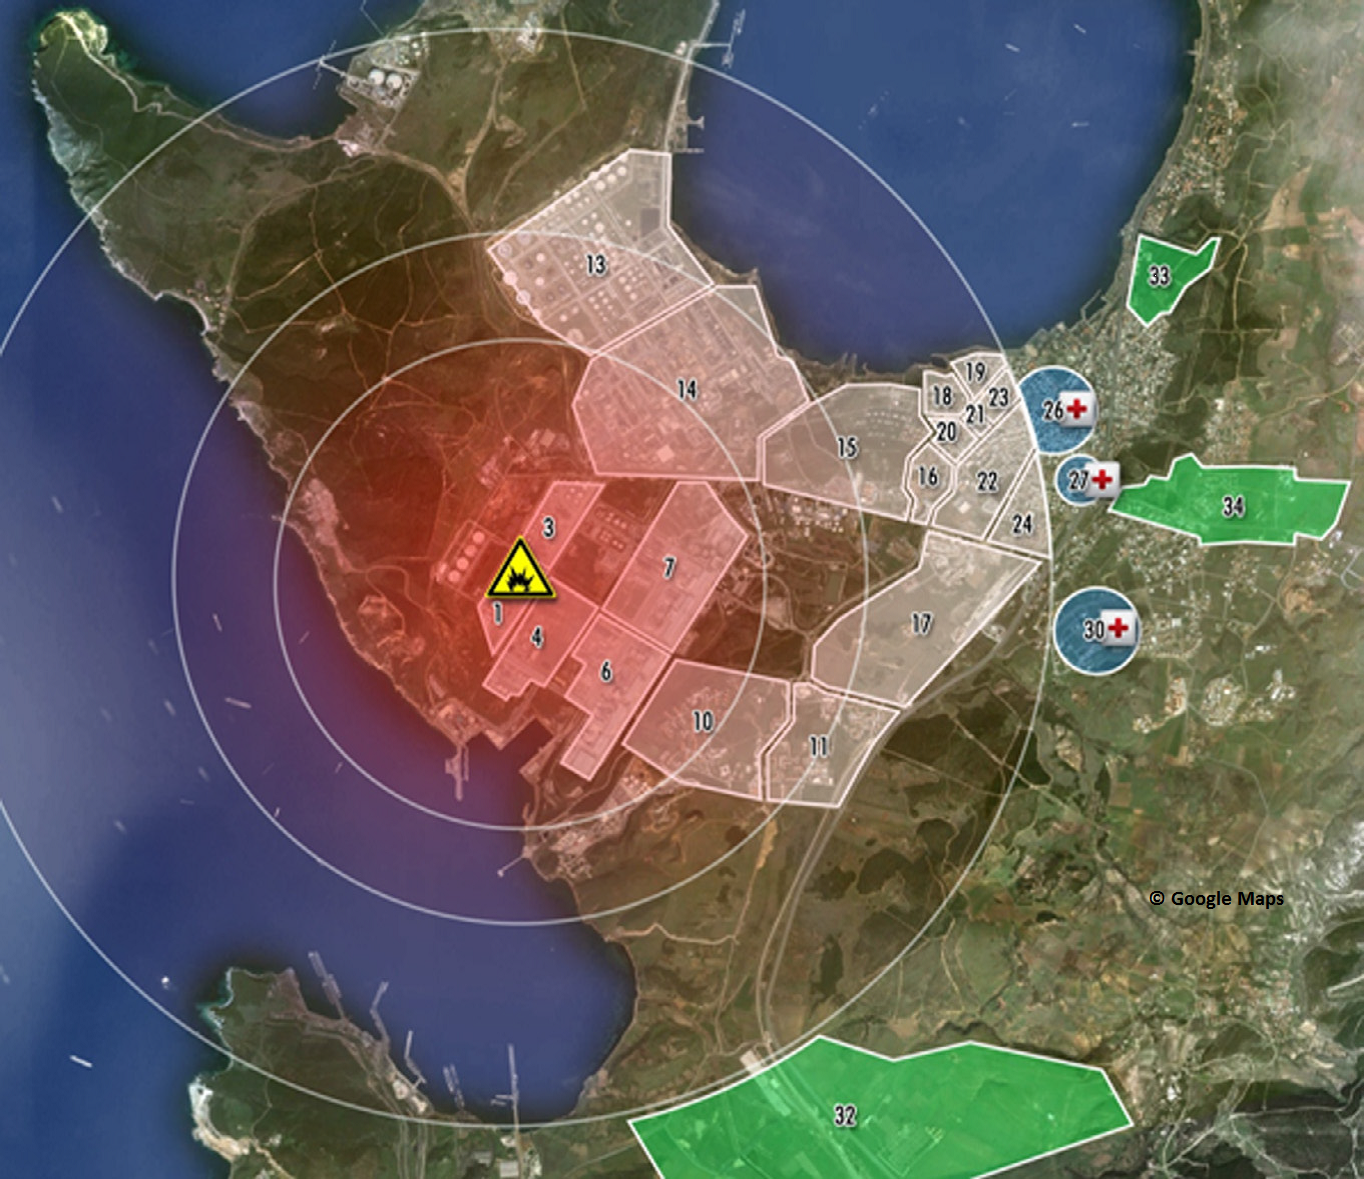
\includegraphics[width=0.8\textwidth, angle=0]{scenarios/figures/aliaga_fig1.png}}%
{}
% ------------

 % ------------
\createfigure%
{MATSim simulation snapshot}%
{MATSim simulation snapshot}%
{\label{fig:aliaga_fig2}}%
{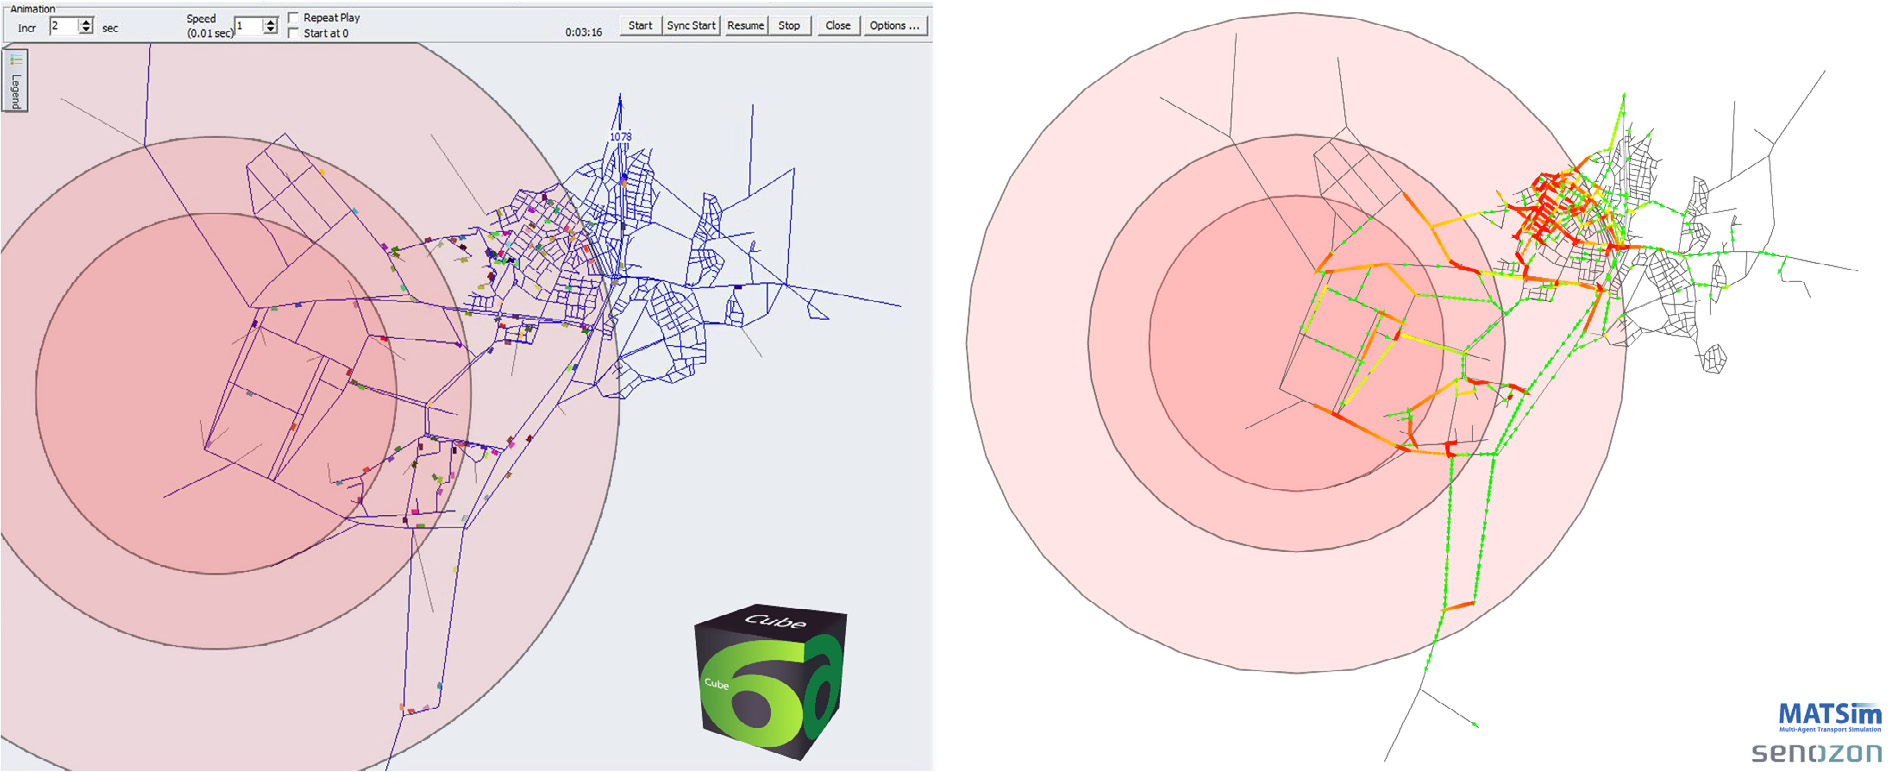
\includegraphics[width=0.8\textwidth, angle=0]{scenarios/figures/aliaga_fig2.png}}%
{}
% ------------

 % ------------
\createfigure%
{OD matrices for evacuation scenarios}%
{OD matrices for evacuation scenarios}%
{\label{fig:aliaga_tab1}}%
{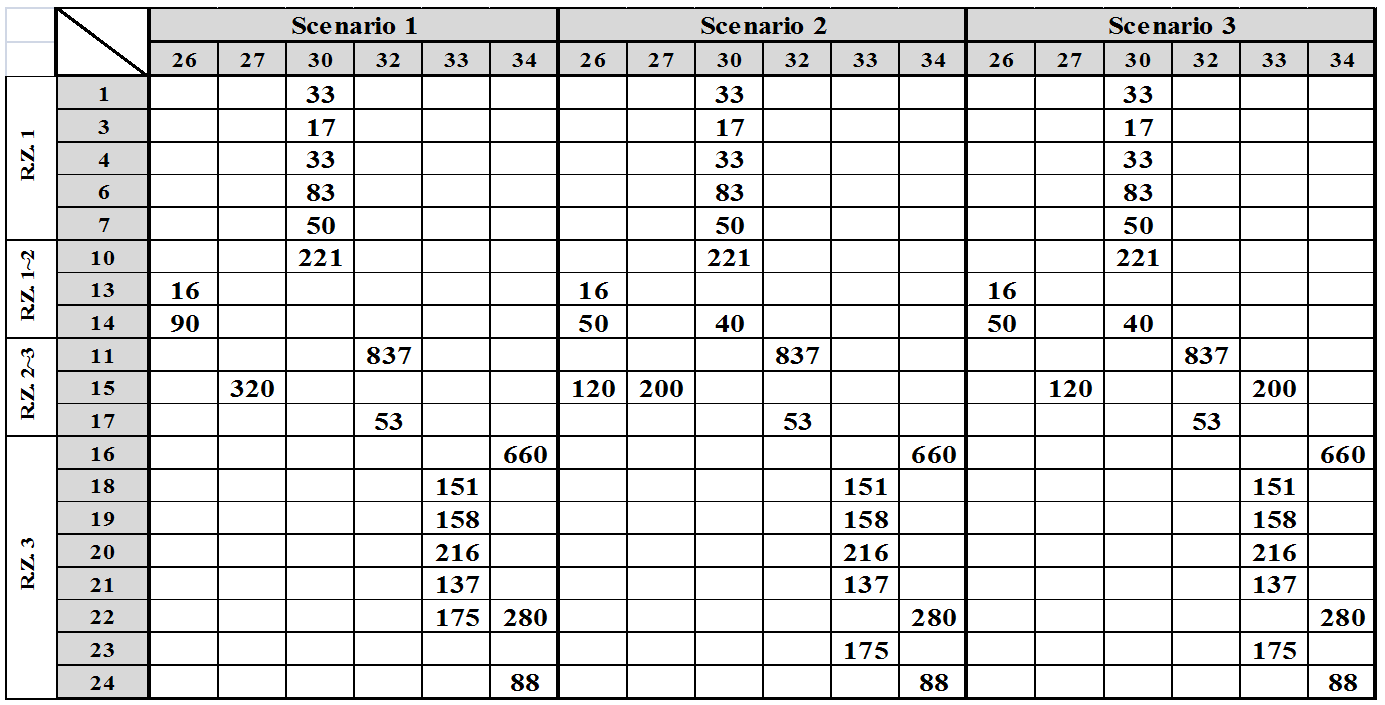
\includegraphics[width=0.8\textwidth, angle=0]{scenarios/figures/aliaga_tab1.png}}%
{}
% ------------

%---------------------------------------------------------------------
\createtable%
{Risk zones evacuation times in minutes}%
{Risk zones evacuation times in minutes}%
{\label{tab:aliaga_tab2}}%
{%
  \begin{tabular}[c]{|l|c|c|c|}
    \hline
		& \textbf{Risk zone~1} & \textbf{Risk zone~2} & \textbf{Risk zone~3} \\
		\hline
    Scenario~1 & 45 & 83 & 86 \\
		Scenario~2 & 44 & 82 & 91 \\
		Scenario~3 & 47 & 86 & 88 \\
    \hline
  \end{tabular}
}%
{}
%---------------------------------------------------------------------

% ##################################################################################################################
